\documentclass{beamer}
\usepackage{color}
\usepackage{subfig}
\usepackage{graphicx}
\usepackage{float}
\usepackage{cite}
\usepackage{bbm}
\usepackage{comment}
%\usepackage[UTF8]{ctex}
\usepackage{tikz}
\usepackage{scalefnt, xr}
\usetikzlibrary{arrows}
\usetikzlibrary{plotmarks}
\usetikzlibrary{overlay-beamer-styles}
\usetikzlibrary{calc}
\usetikzlibrary{scopes}
\usetheme{Madrid}
\usepackage{tikz}
\usetikzlibrary{arrows.meta,decorations.pathmorphing}

\theoremstyle{plain}
\newtheorem{thm}{Theorem}
\newtheorem{cor}[thm]{Corollary}
\newtheorem{lem}[thm]{Lemma}
\newtheorem{prop}[thm]{Proposition}
\newtheorem{remark}[thm]{Remark}
%
\theoremstyle{definition}
\newtheorem{defn}[thm]{Definition}


\colorlet{prp}{red!50!blue!80!white}
\colorlet{Tcol}{blue}
\colorlet{Fcol}{orange!85!red!90!black}
\colorlet{rgr}{red!70!gray}
\colorlet{bgr}{blue!60!gray}
\colorlet{gray}{black!50!white}
\colorlet{lgray}{gray!50!white}
\colorlet{dfc}{green!35!blue!80!gray!90!black}
\colorlet{rfc}{black!45!gray!80!blue!80!white}
\colorlet{rkc}{lightgray}
\colorlet{rsbcol}{green!80!blue!70!gray!70!black}
\colorlet{nbdcol}{red!60!blue!90!gray!90!black}
\newcommand{\BB}{\mathbbm}
\newcommand{\ol}{\overline}
\newcommand{\ul}{\underline}
\newcommand{\op}{\operatorname}
\newcommand{\la}{\langle}
\newcommand{\ra}{\rangle}
\newcommand{\bd}{\mathbf}
\newcommand{\im}{\operatorname{Im}}
\newcommand{\re}{\operatorname{Re}}
\newcommand{\frk}{\mathfrak}
\newcommand{\eqD}{\overset{d}{=}}
\newcommand{\ep}{\varepsilon}
\newcommand{\rta}{\rightarrow}
\newcommand{\xrta}{\xrightarrow}
\newcommand{\Rta}{\Rightarrow}
\newcommand{\hookrta}{\hookrightarrow}
\newcommand{\wt}{\widetilde}
\newcommand{\wh}{\widehat} 
\newcommand{\mcl}{\mathcal}
\newcommand{\pre}{{\operatorname{pre}}}
\newcommand{\lrta}{\leftrightarrow}
\newcommand{\bdy}{\partial} 
\newcommand{\rng}{\mathring}
\newcommand{\srta}{\shortrightarrow}
\newcommand{\el}{l}
\newcommand{\ER}{Erd\H{o}s-R\'{e}nyi}
\newcommand{\tr}{{\mathrm{tr}}}
\newcommand{\LFPP}{{\textnormal{\tiny{\textsc{LFPP}}}}}
\newcommand{\ccM}{{\mathbf{c}_{\mathrm M}}}

\newcommand*\tc[1]{\tikz[baseline=(char.base)]{\node[shape=circle,draw,inner sep=1pt] (char) {#1};}}
\newcommand*\tb[1]{\tikz[baseline=(char.base)]{\node[shape=rectangle,draw,inner sep=2.5pt] (char) {#1};}}

%Remove spacing before \left and \right
\let\originalleft\left
\let\originalright\right
\renewcommand{\left}{\mathopen{}\mathclose\bgroup\originalleft}
\renewcommand{\right}{\aftergroup\egroup\originalright}



\newcommand{\post}[2]{\begin{center} \includegraphics[width=#2]{#1} \end{center} }
\newcommand{\scite}[1]{\textcolor{blue}{\scriptsize [#1]}}

%Information to be included in the title page:
\title[Diameter of PAM]{Asymptotic Diameter of Preferential Attachment Model}
\author{Shuyang Gong and Zhangsong Li}
\institute[]{School of Mathematical Sciences, Peking University}
\date[May 2025]{May 29, 2025\\ \medskip\bigskip\bigskip Joint work with Hang Du (MIT) and Haodong Zhu (TU/E)\\ \medskip\bigskip\bigskip
{\color{bgr}YMSC Probability Seminar} }


\begin{document}

\frame{\titlepage}

\begin{frame}
\frametitle{Preferential attachment model (PAM)}
At each time $t$, a new vertex labeled $t$ arrives and forms $m$ edges, one at a time, to existing nodes $v \in [t-1]$:
\begin{align*}
    \mathbb P(t \to v) \varpropto \operatorname{deg}(v)+\delta \mbox{ where } \delta>-m  \,.
\end{align*}
\begin{figure}
    \begin{center}
    \only<1>{\post{PAM_Step1.jpg}{2in}}
    \only<2>{\post{PAM_Step2.jpg}{2in}}
    \only<3>{\post{PAM_Step3.jpg}{2in}}
    \only<4>{\post{PAM_Step4.jpg}{2in}}
    \only<5>{\post{PAM_Step5.jpg}{2in}}
    \end{center}
\end{figure}
\end{frame}





\begin{frame}
\frametitle{Preferential attachment model (PAM)}
At each time $t$, a new vertex labeled $t$ arrives and forms $m$ edges, one at a time, to existing nodes $v \in [t-1]$:
\begin{align*}
    \mathbb P(t \to v) \varpropto \operatorname{deg}(v)+\delta \mbox{ where } \delta>-m  \,.
\end{align*}
\begin{itemize}
    \item $\operatorname{deg}(v)$ is updated after each edge is added
    \item \pause $\delta=\infty$: uniform-attachment (no degree preference)
    \item \pause $\delta=0$: Barab\'{a}si-Albert model {\color{rgr}[Barab\'{a}si-Albert'99]}
    \item \pause The {\color{bgr}smaller} $\delta$, the {\color{bgr}stronger} preference for high-degree vertices
    \item \pause A popular {\color{bgr}dynamical} model that shares many similar features as in empirically studied real-world networks.
\end{itemize}
\end{frame}





\begin{frame}
\frametitle{Features of PAM: Power-law degree distribution}
\begin{thm}[Bollob\'as-Riordan-Spencer-Tusn\'ady'01, Deijfen-van den Esker-van der Hofstad-Hooghiemstra'09]
    PAM with parameter $m,\delta$ yields power-law degree sequence with exponent $\tau=3+\delta/m>2$.
\end{thm}
\pause
\begin{columns}
    \begin{column}{0.5\textwidth}
        \begin{figure}
        \begin{centering}
        \post{Degree_Distribution.jpeg}{2in}
        \caption{degree sequences in PAM with $m=2,\delta=0,\tau=3,n=10^6$ (picture courtesy of Remco van der Hofstad)}
        \end{centering}
        \end{figure}
    \end{column}
    \begin{column}{0.5\textwidth}
        \begin{figure}
        \begin{centering}
        \post{Degree_Real_Network.jpeg}{1.5in}
        \caption{degree sequences in Internet Movie Data Base 2007 {\color{red}[Britton-Deijfen-L\H{o}f'2007]} }
        \end{centering}
        \end{figure}
    \end{column}
\end{columns}
\end{frame}





\begin{frame}
\frametitle{Features of PAM: Small world phenomenon}
\begin{columns}
    \begin{column}{0.5\textwidth}
        \begin{figure}
        \begin{centering}
        \post{Six_Degree_Separ.jpeg}{1.4in}
        \caption{Six degrees of separation: ``{\color{bgr}Everybody} on this planet is separated only by six other people''.}
        \end{centering}
        \end{figure}
    \end{column}
    \begin{column}{0.5\textwidth}
        \begin{figure}
        \begin{centering}
        \post{Dist_Real_Network.jpeg}{1.8in}
        \caption{Distances in social networks \emph{Livejournal} {\color{red}[Backstrom-Boldi-Rosa-Ugander-Vigna'2010]} }
        \end{centering}
        \end{figure}
    \end{column}
\end{columns}
\begin{itemize}
    \item \pause \underline{Question}: Can we rigorously justify the small world phenomenon in PAM?
    \item \pause Equivalently, does PAM have small {\color{bgr}diameters}?
\end{itemize}
\end{frame}





\begin{frame}
\frametitle{Previous results on diameters of PAM}
\quad average degree: $2m$; \quad\quad $\mathbb P(t\to v)\varpropto \operatorname{deg}(v)+\delta$;
\begin{itemize}
    \item \pause {\color{rgr}[Pittel'94]}: the diameter of PAM with $m=1,\delta>-1$ is typically 
    \[
    (1+o(1))\tfrac{2(1+\delta)\log n}{(2+\delta)\theta} \,,
    \]
    where $\theta \in (0,1)$ is the solution to $\theta+(1+\delta)(1+\log\theta) = 0$.
    \item \pause {\color{rgr}[Bollob\'as-Riordan'09]}: the diameter of PAM with $m\geq 2,\delta=0$ is typically $(1+o(1))\tfrac{\log n}{\log\log n}$.
    \item \pause {\color{rgr}[Caravenna-Garavaglia-van der Hofstad'19]}: the diameter of PAM with $m\geq 2,-m<\delta<0$ is typically 
    \[
    (1 + o(1)) \left( \tfrac{4}{|\log(1 + \delta/m)|} + \tfrac{2}{\log m} \right) \log\log n \,.
    \]
    \item \pause Remaining case: PAM with ${\color{bgr}m\geq 2, \delta>0}$.
\end{itemize}
\end{frame}





\begin{frame}
\frametitle{PAM with $m\geq 2,\delta>0$}
\quad average degree: $2m$; \quad\quad $\mathbb P(t\to v)\varpropto \operatorname{deg}(v)+\delta$; 
\begin{itemize}
    \item \pause Difficulties for extending previous argument:
    \begin{itemize}
        \item \pause $m\geq 2 \Longrightarrow$ no tree structure;
        \item \pause $\delta>0 \Longrightarrow$ no hub structure.
    \end{itemize}
    \item \pause Difficulties in the model:
    \begin{itemize}
        \item \pause Lack of independence;
        \item \pause Harder to couple to the local limit.
    \end{itemize}
    \item \pause {\color{rgr}[Dommers-van der Hofstad-Hooghiemstra'10]}: the diameter of PAM with $m\geq 2,\delta>0$ is typically $O(\log n)$. 
\end{itemize}
\end{frame}





\begin{frame}
\frametitle{Typical distance of PAM with $m\geq 2,\delta>0$}
average degree: $2m$; \quad $\mathbb P(t\to v)\varpropto \operatorname{deg}(v)+\delta$; \quad $\operatorname{PA}^{(m,\delta)}_n$: law of PAM
\begin{thm}[van der Hofstad-Zhu'25+]
    Let $\nu$ to be the exponential growth parameter of the local limit of the preferential attachment model, then
    \[
        \mathbb P_{G \sim \operatorname{PA}^{(m,\delta)}_n} \mathbb P_{u,v \sim \operatorname{unif}(V(G))}\big( \operatorname{dist}_G(u,v)=(1+o(1))\log_\nu n \big) = 1-o(1) \,,
    \] 
\end{thm}
\begin{itemize}
    \item \pause Implies that typically we have $\operatorname{dist}_G(u,v)=(1+o(1))\log_\nu n$ for $\geq 99\%$ vertex pairs (thus typically $\operatorname{diam}(G)\geq (1+o(1))\log_\nu n$).
    \item \pause Relies on first/second moment method + path counting technique.
    \item \pause Conjecture in {\color{rgr}[van der Hofstad-Zhu'25+]}: typically the diameter of PAM with $m\geq 2,\delta>0$ is also $(1+o(1))\log_{\nu} n$.
\end{itemize}
\end{frame}





\begin{frame}
\frametitle{Our result: from typical distance to diameter}
average degree: $2m$; \quad $\mathbb P(t\to v)\varpropto \operatorname{deg}(v)+\delta$; \quad $\operatorname{PA}^{(m,\delta)}_n$: law of PAM
\begin{thm}[Du-G.-L.-Zhu'25+]
    \begin{itemize}
        \item Let $M_n=M_n(G)$ be the median of pairwise vertex distances of $G \sim \operatorname{PA}^{(m,\delta)}_n$.
        \item Let $R_n = R_n(G)$ satisfying $\#\{ R_n \mbox{-neighborhood of } u \} \geq (\log n)^2$ for all $u \in V(G)$. 
    \end{itemize} 
    Then we have $\mathbb P_{G \sim \operatorname{PA}^{(m,\delta)}_n}(\operatorname{diam}(G) \leq M_n+O(1)\cdot R_n)=1-o(1)$.
\end{thm}
\begin{itemize}
    \item \pause Note that {\color{rgr}[van der Hofstad-Zhu'25+]} implies that typically $M_n(G)=(1+o(1))\log_\nu n$.
    \item \pause {\color{rgr}[Du-G.-L.-Zhu'25+]}: typically $R_n(G)\leq (\log n)^{\frac{2}{3}}$. {\color{bgr}(expected to be far from tight)}.
    \item \pause Conclusion: typically $\operatorname{diam}(G) \leq  (1+o(1))\log_\nu n$.
\end{itemize}
\end{frame}





\begin{frame}
\frametitle{Discussions: from typical distance to diameter}
It seems that our result 
\[
{\color{bgr} \operatorname{diam}(G) \leq M_n(G)^{\leftarrow\text{average distance}}  +O(1)\cdot R_n(G)^{ \leftarrow \text{depth for large neighborhood} }  }
\]
holds for many interesting cases beyond the scope of PAM, e.g.
\begin{itemize}
    \item\pause Random $d$-regular graph ($d \geq 3$): 
    \begin{itemize}
        \item\pause {\color{rgr}[Chung-Lu'02]}: $M_n=\log_{d-1} n+O(\log\log n)$;
        \item\pause $R_n=O(\log\log n)$;
        \item\pause {\color{rgr}[Bollob\'as-Fernandez De La Vega'81]}: $\operatorname{diameter}=\log_{d-1} n+O(\log\log n)$.
    \end{itemize}
    \item\pause Giant component of Erd\H{o}s-R\'{e}nyi graph with average degree $\lambda=1+\Omega(1)$:
    \begin{itemize}
        \item\pause {\color{rgr}[Riordan-Wormald'08]}: $M_n=c(\lambda)\log n$;
        \item\pause $R_n=\Theta(1)\cdot\log n$;
        \item\pause {\color{rgr}[Fernholz-Ramachandran'07]} (see also {\color{rgr}[Ding-Kim-Lubetzky-Peres'10]} for more general $\lambda$): $\operatorname{diameter}=(1+\Theta(1))\cdot \text{average distance}$.
    \end{itemize}
\end{itemize}
\end{frame}

\begin{frame}{Proof idea}
\footnotesize
\begin{itemize}
    \item\pause \textcolor{blue}{Two random sources: }denote $\operatorname{PA}(\cdot)$ the distribution of $G_n$ and $\mathbb P_{u,v}$ the uniform selection.
    \item\pause Let $M_n$ be the upper bound of \textcolor{blue}{``typical" median distance}: with prob. $1-o(1)$ over $\operatorname{PA}$ on $G_n$
    \begin{equation}
        \mathbb P_{u,v\sim \operatorname{UNIF}(V(G_n))}\big[\operatorname{dist}(u,v)\leq M_n\,|\,G_n\big]\geq 1/2\,.\notag
    \end{equation}
    \begin{itemize}
        \item By \textcolor{red}{[van der Hofstad and Zhu 25]}, we can take $M_n=(1+o(1))\log_\nu n$.
    \end{itemize}
    \item\pause \textcolor{blue}{\textbf{High level idea}}: $\forall u,v$, with probability $1-o(1/n^2)$, there exists two vertices in their respective $R_n$-neighborhoods with distance at most $M_n$.
    % ——————————————————————
% TikZ figure: two R_n–neighbourhoods (as triangles) and an M_n path
% ——————————————————————
\begin{figure}[h]
\centering
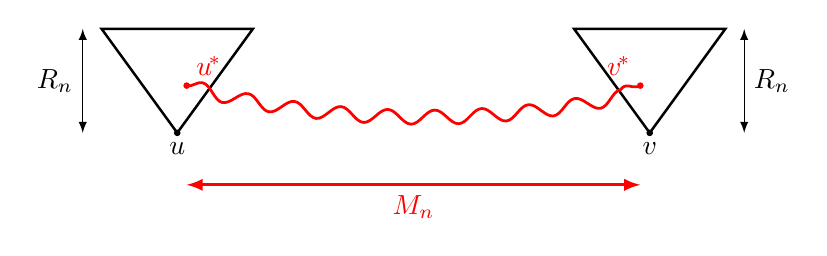
\begin{tikzpicture}[xscale=0.6,yscale=0.6,>=latex]
% — styles ––––––––––––––––––––––––––
\tikzstyle{neigh}    =[line width=0.9pt]
\tikzstyle{pathblue}=[red,line width=1pt]

% --- key coordinates ------------------------------------------
\coordinate (u) at (0,0);        % left outer vertex
\coordinate (v) at (10,0);       % right outer vertex

% left triangle apexes
\coordinate (ul) at (-1.6,2.2);
\coordinate (ur) at ( 1.6,2.2);
% right triangle apexes
\coordinate (vl) at (8.4,2.2);
\coordinate (vr) at (11.6,2.2);

% --- draw neighbourhood cones ---------------------------------
\draw[neigh] (u) -- (ul) -- (ur) -- cycle;
\draw[neigh] (v) -- (vl) -- (vr) -- cycle;

% boundary vertices + labels
\fill (u) circle(2pt) node[below]{$u$};
\fill (v) circle(2pt) node[below]{$v$};

% --- vertical R_n arrows --------------------------------------
\draw[<->] (u)+(-2,0) -- ++(-2,2.2) node[midway,left]{$R_n$};
\draw[<->] (v)+( 2,0) -- ++(2,2.2) node[midway,right]{$R_n$};

% --- interior points & labels ---------------------------------
\coordinate (ustar) at (0.2,1);
\coordinate (vstar) at (9.8,1);
\fill[red] (ustar) circle(2pt) node[red,above right]{$u^{\!*}$};
\fill[red] (vstar) circle(2pt) node[red,above left]{$v^{\!*}$};

% --- blue wiggly path -----------------------------------------
\draw[pathblue,decorate,decoration={snake,amplitude=0.9mm,segment length=6mm}] (ustar) .. controls (3,0.2) and (7,0.2) .. (vstar);

% --- overall M_n arrow below ----------------------------------
\draw[pathblue,<->] (ustar |-, -1.1) -- (vstar |-, -1.1) node[midway,below]{$M_n$};

\end{tikzpicture}
%\caption{Illustration of two $R_n$–neighborhoods around vertices $u$ and $v$, and a connecting path of length $M_n$.}
\end{figure}
  %  \begin{figure}
   %     \centering
    %    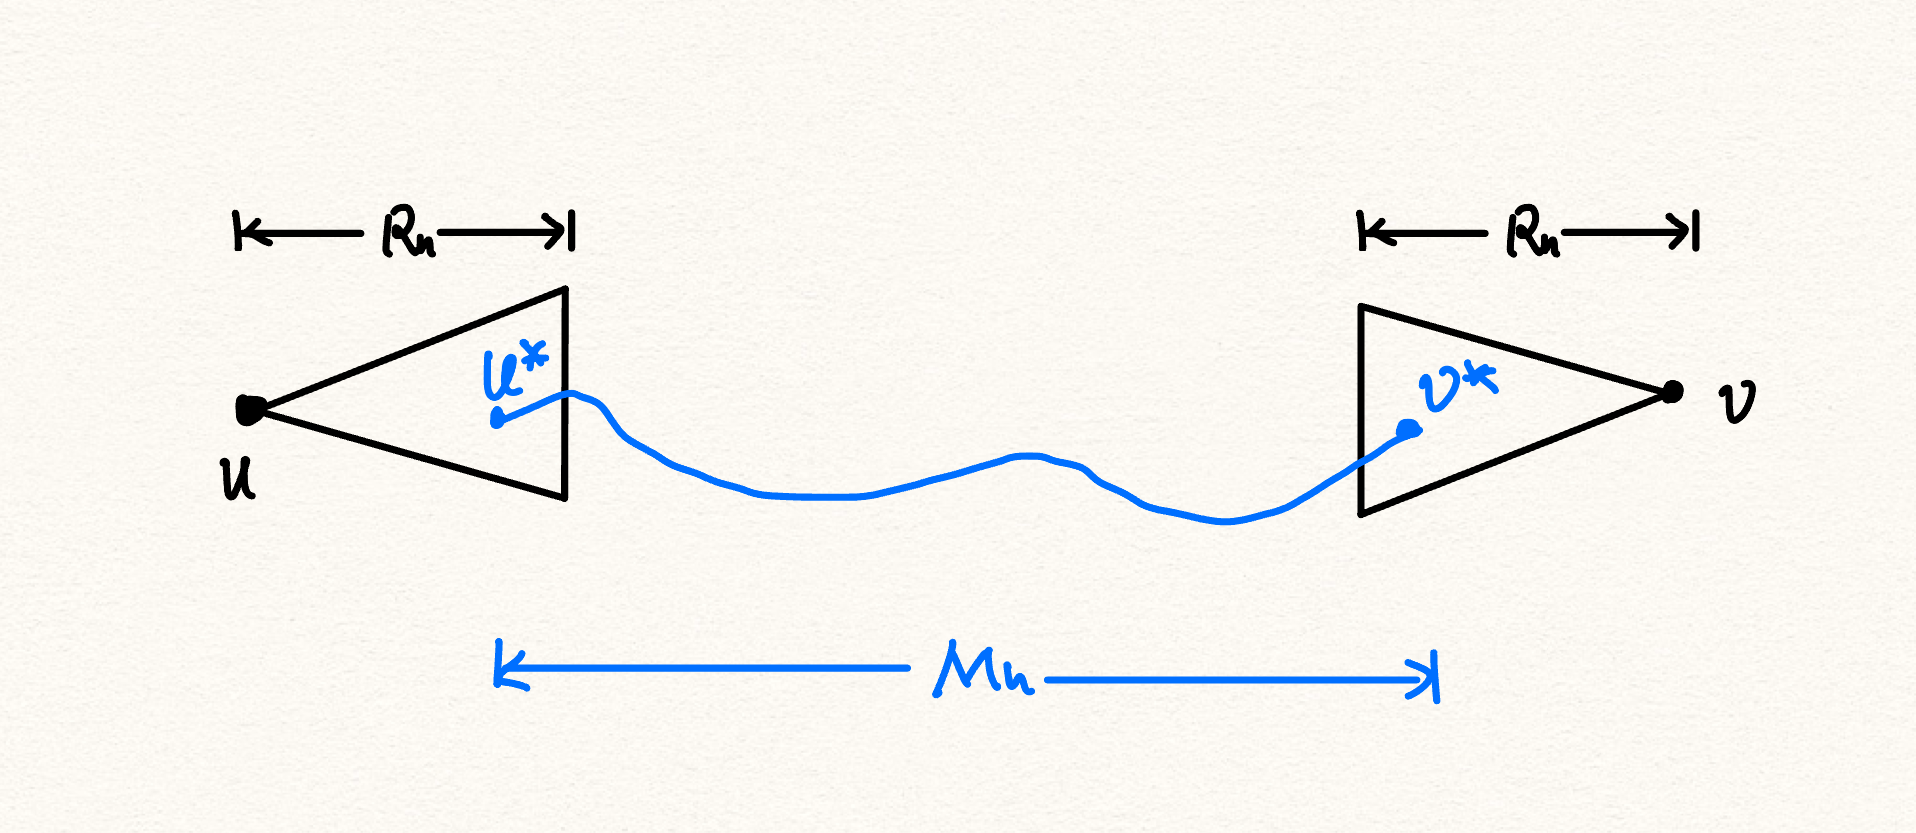
\includegraphics[width=0.5\linewidth]{two_neighborhoods.jpg}
        %\caption{Caption}
        %\label{fig:enter-label}
   % \end{figure}
    \item\pause Diameter at most $M_n+2R_n$. $M_n= \log_\nu n,R_n=o(\log n)$.  
\end{itemize}
\end{frame}

\begin{frame}{Uniform growth of neighborhood size}
\begin{lemma}
    Taking $R_n=(\log n)^{2/3}$, 
    \begin{equation}
        \operatorname{PA}\left[|\operatorname{N}_{R_n}(u)|\geq (\log n)^4,\forall u\in V(G_n)\right]=1-o(1)\,.\notag
    \end{equation}
\end{lemma}
   \begin{itemize}
       \item\pause \textcolor{blue}{Far from tight.} Expected to be $R_n=O(\log\log n)$ for $|\operatorname{N}_{R_n}(u)|\geq \operatorname{polylog}(n)$. 
       \begin{itemize}
           \item\pause $m\geq 2$ condition $\Rightarrow$ exponential growth in neighborhood size.
       \end{itemize}
       \item\pause \textcolor{blue}{Major Challenge:} dealing with dependence issue.
       \begin{itemize}
           \item \begin{lemma}[Conditional attachment lemma]
       Let $E$ be a set of potential edges in $G_n\sim\operatorname{PA}$ and $A$ be a set of vertices. Assume that $A\subset [ s,n]$, then 
    \begin{equation}
    \operatorname{PA}[u\to A\mid E\subset E(G_n)]\le \frac{|A|(m+\delta+1)+|E|}{(2s-2)m+s\delta}\,.\notag
    \end{equation}
   \end{lemma}
       \end{itemize}
   \end{itemize}
\end{frame}

\begin{frame}{Key ingredient: typical vertices}
    \begin{itemize}
        \item\pause \textbf{\textcolor{blue}{Typical vertices}}: for any $u$, let $\mathcal{A}(u)$ denote the set of vertices $w$ with $\operatorname{dist}(u,w)\leq M_n$. $u$ is called \textcolor{blue}{typical} if $|\mathcal{A}(u)|\geq n/10$.
        \item\pause With prob. $1-o(1)$, $\#\{\text{typical vertices}\}\geq n/10$. Denoted by $\mathcal{G}_1$.
        \begin{itemize}
            \item\pause \textcolor{red}{[van der Hofstad-Zhu'25]} implies 
            \begin{equation}
               \widetilde{\mathcal{G}}_1\triangleq \Big\{G_n: \mathbb P_{u,v\sim \operatorname{unif}^{\otimes 2}}[\operatorname{dist}_{G_n}(u,v)\leq M_n\,|\,G_n]\geq 1/2\Big\}\,.\notag
            \end{equation}
            holds w.p. $1-o(1)$.
            \item\pause We have $\widetilde{\mathcal{G}}_1\subset \mathcal{G}_1$. Assuming $\mathcal{G}_1^c$ ,
            \begin{equation}
            \begin{split}
                &\mathbb P_{u,v}[\operatorname{dist}_{G_n}(u,v)\leq M_n\,|\,G_n] \\
                \leq& \mathbb P_u[u \text{ is typical}\,|\,G_n]+\mathbb P_{u,v}[u \text{ is not typical}, \operatorname{dist}(u,v)\leq M_n\,|\,G_n]\\
                \leq&\frac{1}{10}+\frac{1}{10}<1/2.
            \end{split}\notag
            \end{equation}
        \end{itemize}
        \item\pause $\Rightarrow$ $\operatorname{PA}(\mathcal{G}_1)=1-o(1)$ under $\operatorname{PA}$.
    \end{itemize}
\end{frame}

%\begin{frame}{Bridging the gap by sprinkling}
 %   \begin{itemize}
  %      \item Breaking $[0,n]$ into three sets: $G_{n-2K_n}\triangleq [1,n-2K_n]$, $I_1\triangleq [n-2K_n,n-K_n]$ and $I_2\triangleq [n-K_n,n]$ where $K_n=n/\log n$.
   %     \item Denote $\mathcal{G}_0$ the neighborhood size event in $G_{n-2K_n}$, and $\mathcal{G}_1$ as the event there are $\geq n/10$ typical vertices in $G_{n-2K_n}$. 
   % \end{itemize}
%\end{frame}
\begin{frame}{Bridging the gap by sprinkling}
\footnotesize
    \begin{itemize}
        \item Breaking $[1 ,n]$ into three sets: $G_{n-2K_n}\triangleq [1,n-2K_n]$, $I_1\triangleq [n-2K_n,n-K_n]$ and $I_2\triangleq [n-K_n,n]$ where $K_n=n/\log n$.
        %\item Denote $\mathcal{G}_0$ the neighborhood size event in $G_{n-2K_n}$, and $\mathcal{G}_1$ as the event there are $\geq n/10$ typical vertices in $G_{n-2K_n}$. 
        \item There exists a $w_1$ in $I_1$, such that $w_1\to \text{ a typical vertex}$ and $w_1\to N_{R_n}(u)$, with probability
           $
             	1-\big(1-O((\log n)^4/n)\big)^{K_n} = 1-\exp\big(-O((\log n)^3)\big)
            $.
         % \item Suppose $w_1\to t^*$, $|\mathcal A(t^*)|\geq n/10$. 
          %\item Use again $\mathcal G_0$ for $v$, there exists $w_2\in I_2$ such that $w_2\to \mathcal A(t^*)$ and $w_2\to N_{R_n}(v)$.
          \item  For any $u,v \in [1,n-2K_n]$, $\operatorname{dist}_{G_n}(u,v)\leq M_n+2R_n+4$ with prob. $1-o(1/n^2)$.
                
    \end{itemize}
    
    \vspace{2mm}
    \centering
    \only<1>{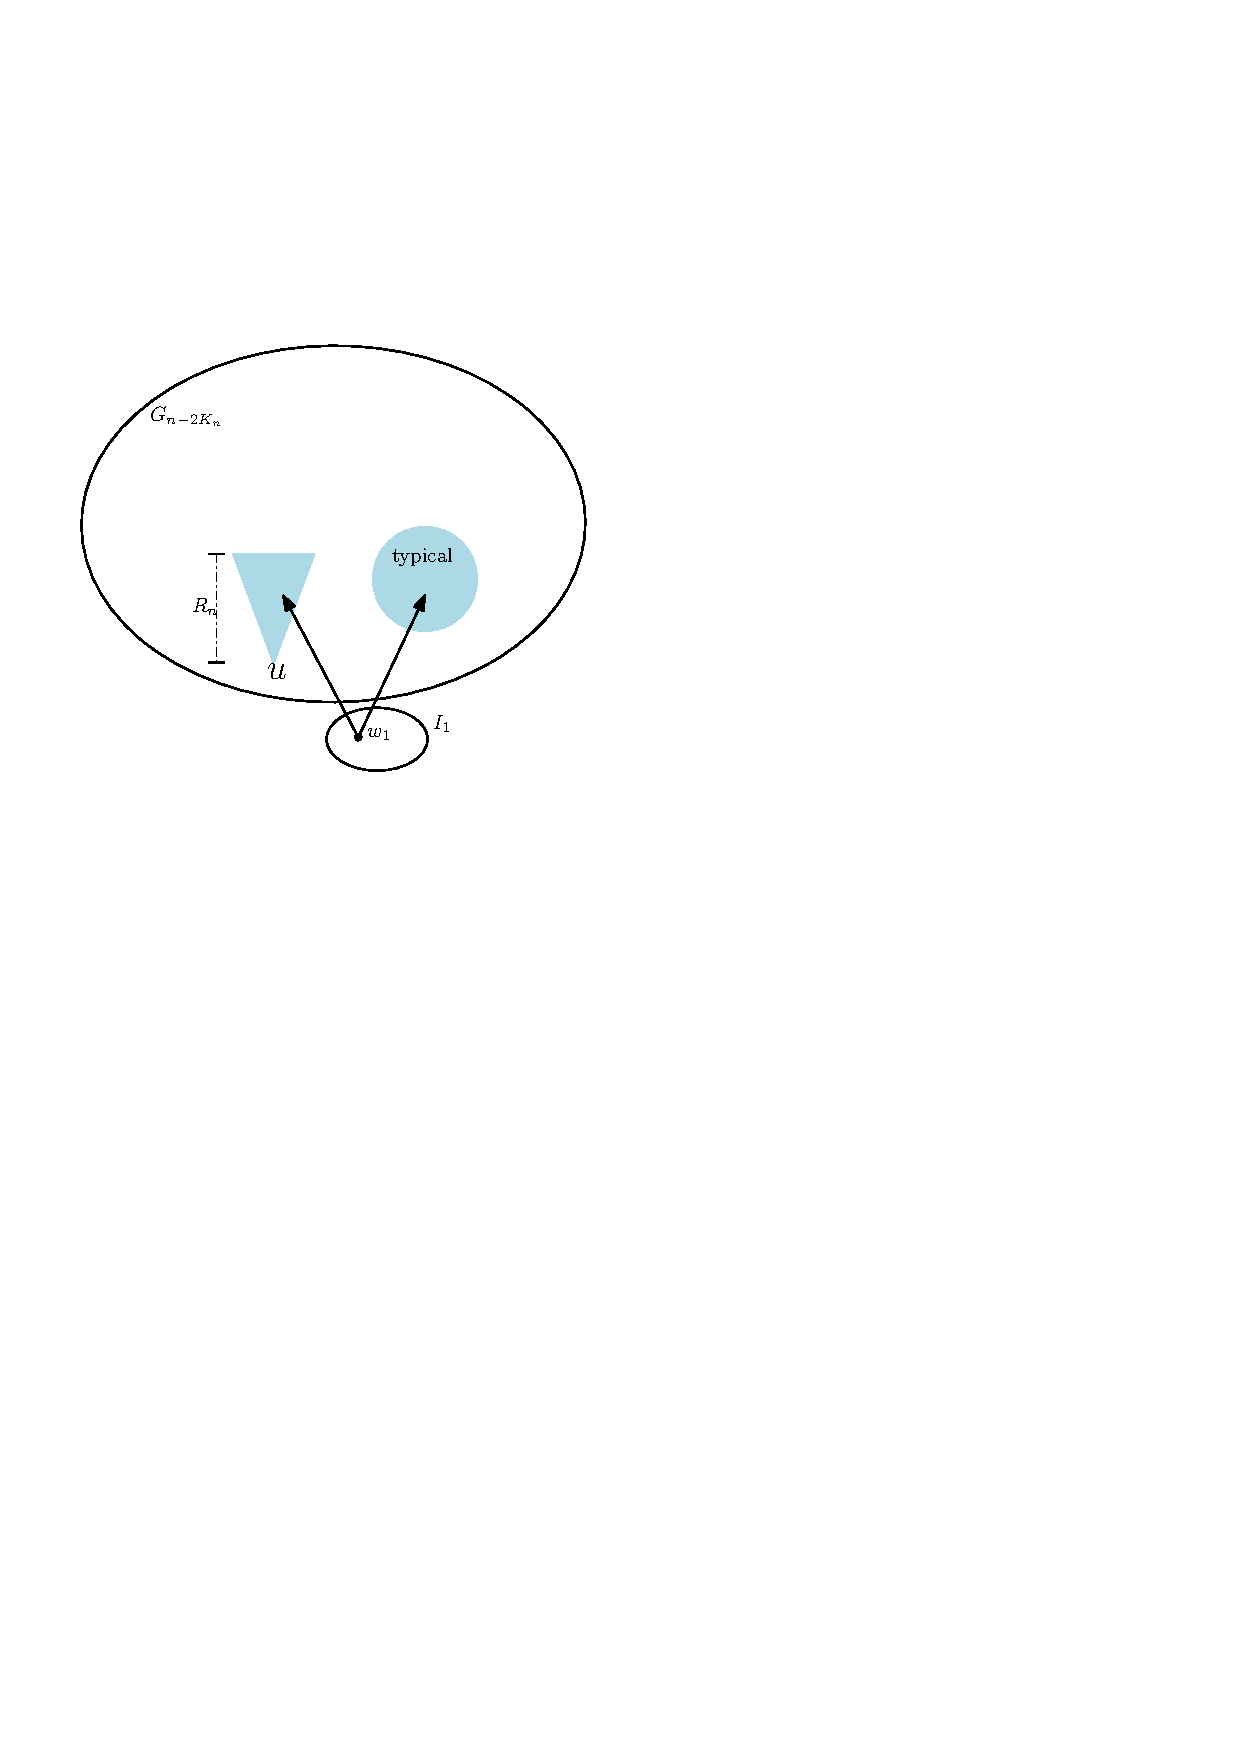
\includegraphics[width=.4\linewidth]{n_minus_2K_1.pdf}}
    
    \only<2>{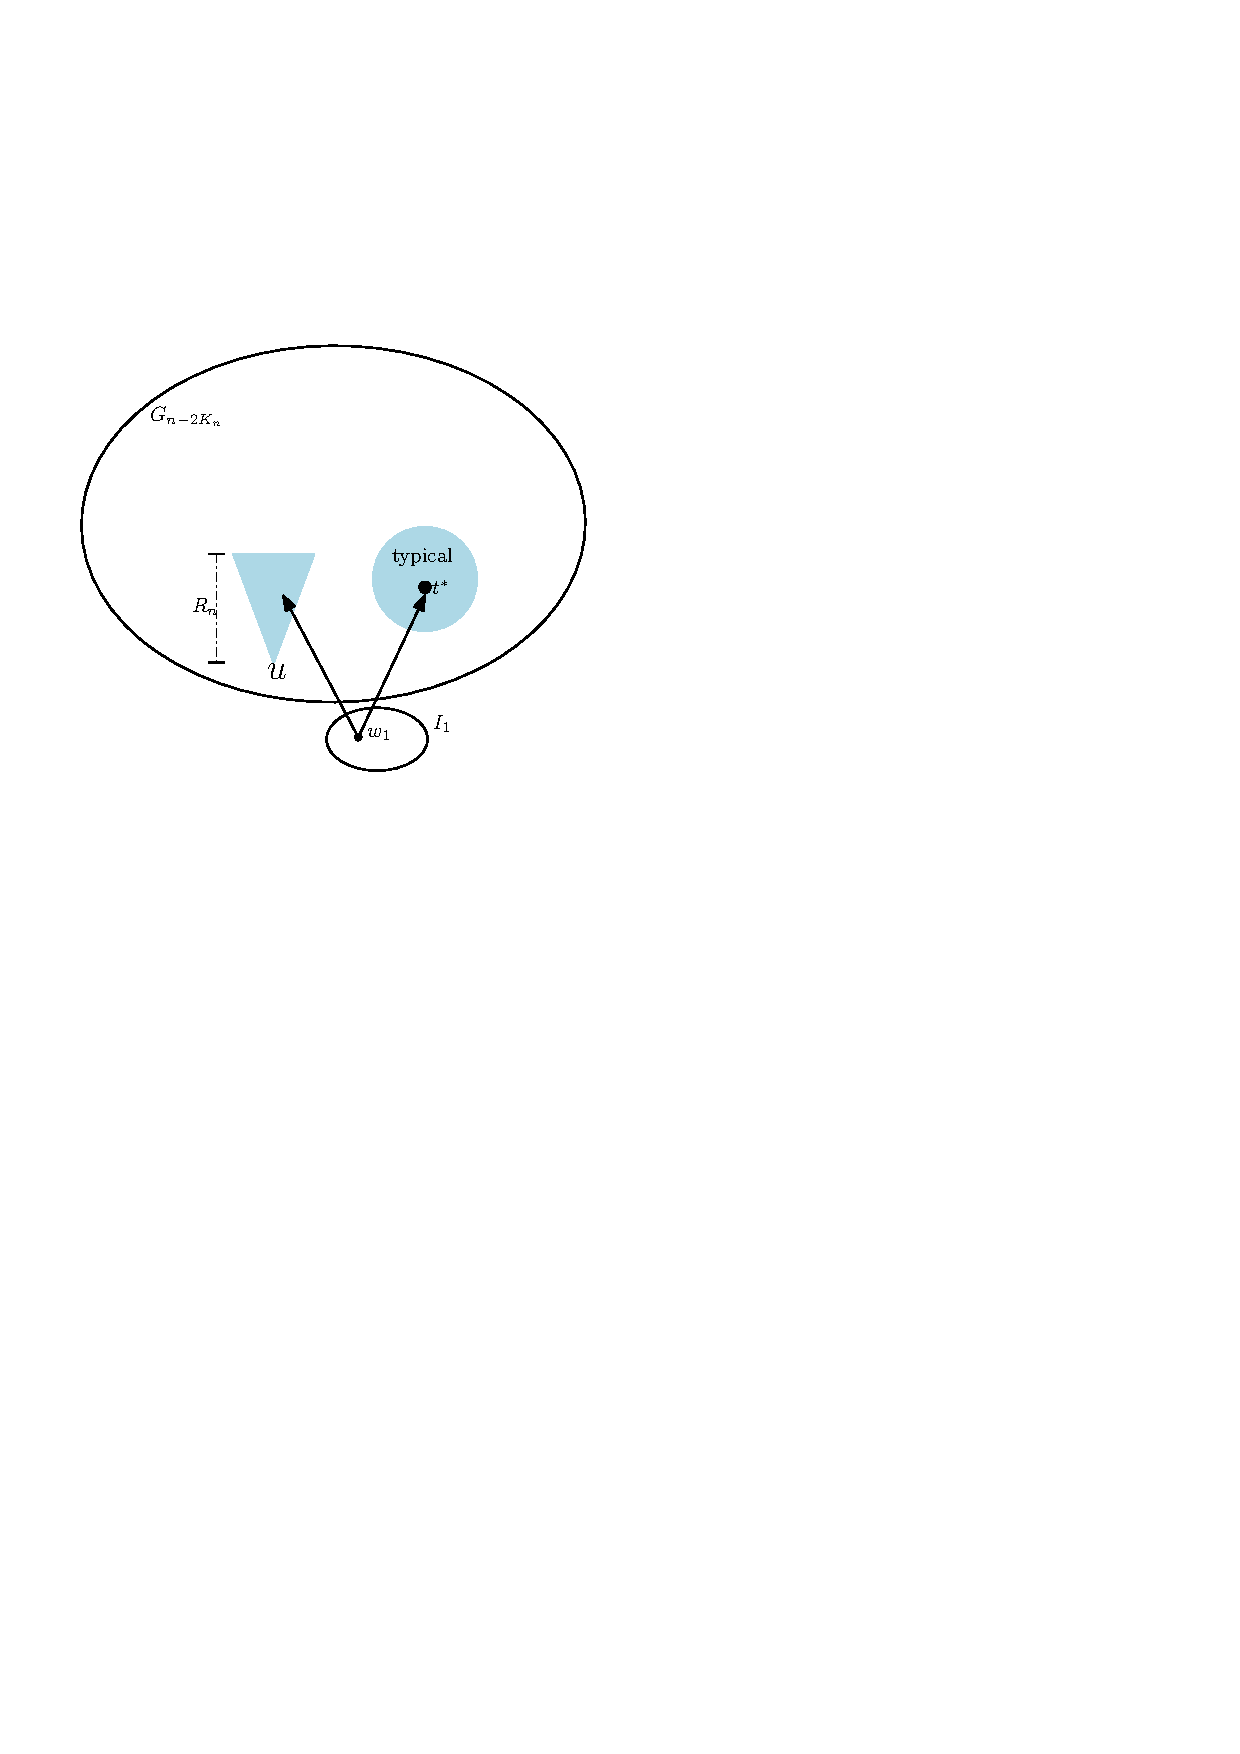
\includegraphics[width=.4\linewidth]{n_minus_2K_2.pdf}}
    
    \only<3>{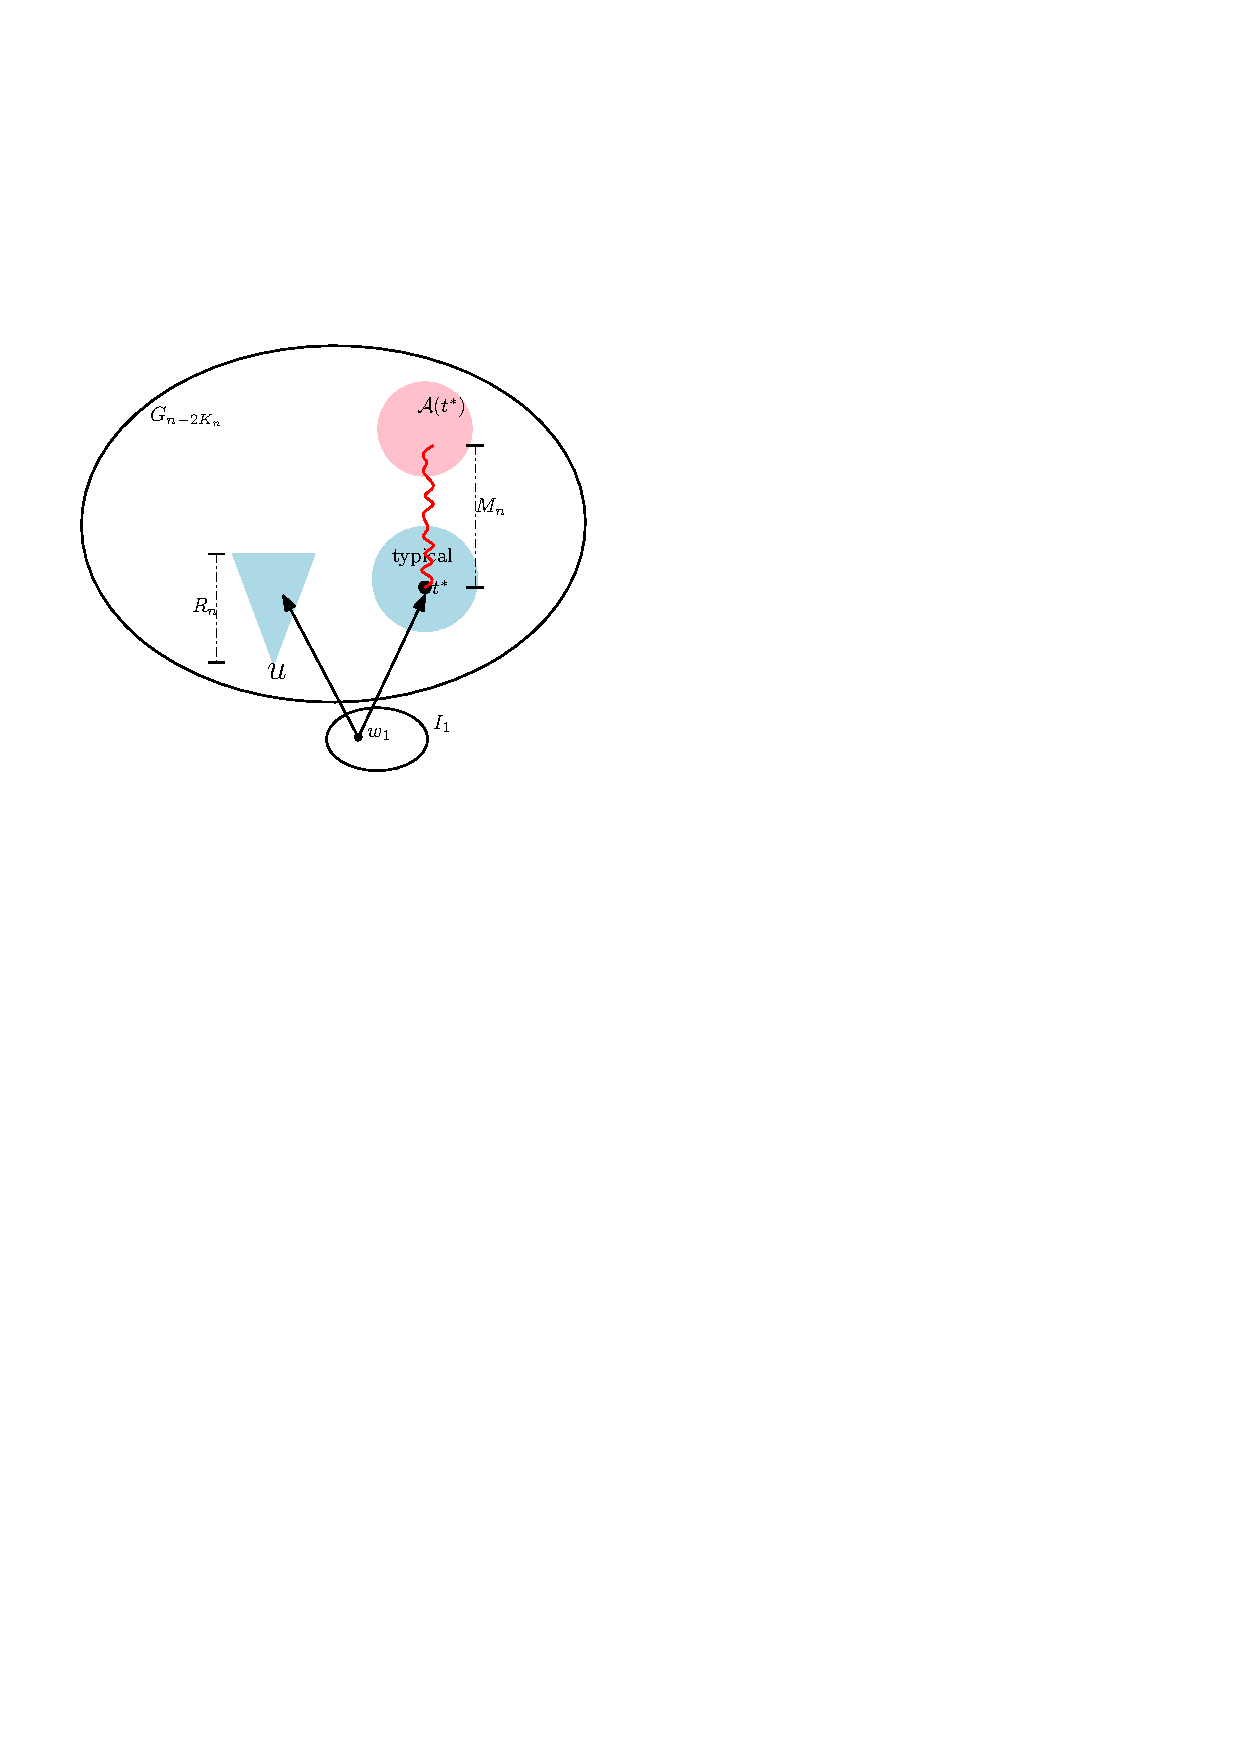
\includegraphics[width=.4\linewidth]{n_minus_2K_3.pdf}}
    
    \only<4>{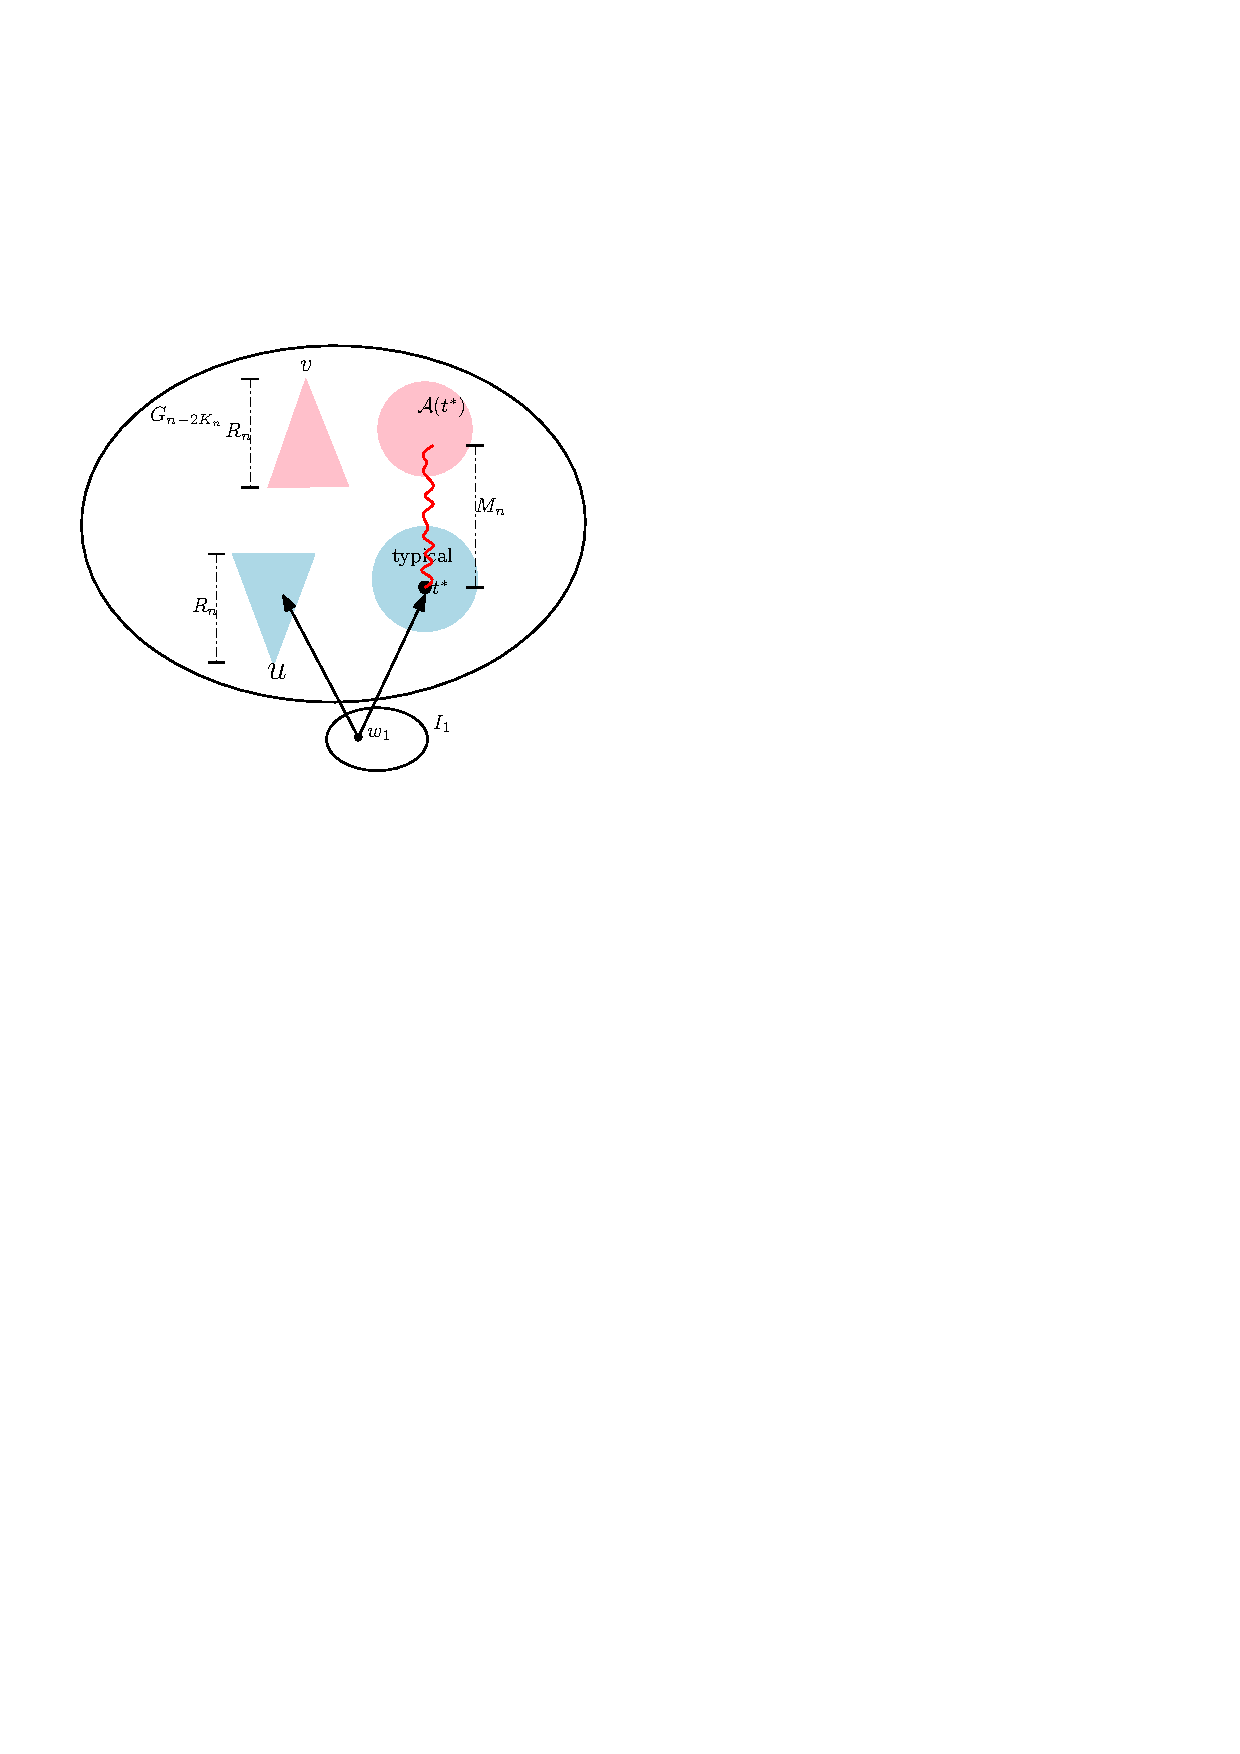
\includegraphics[width=.4\linewidth]{n_minus_2K_4.pdf}}
    
    \only<5>{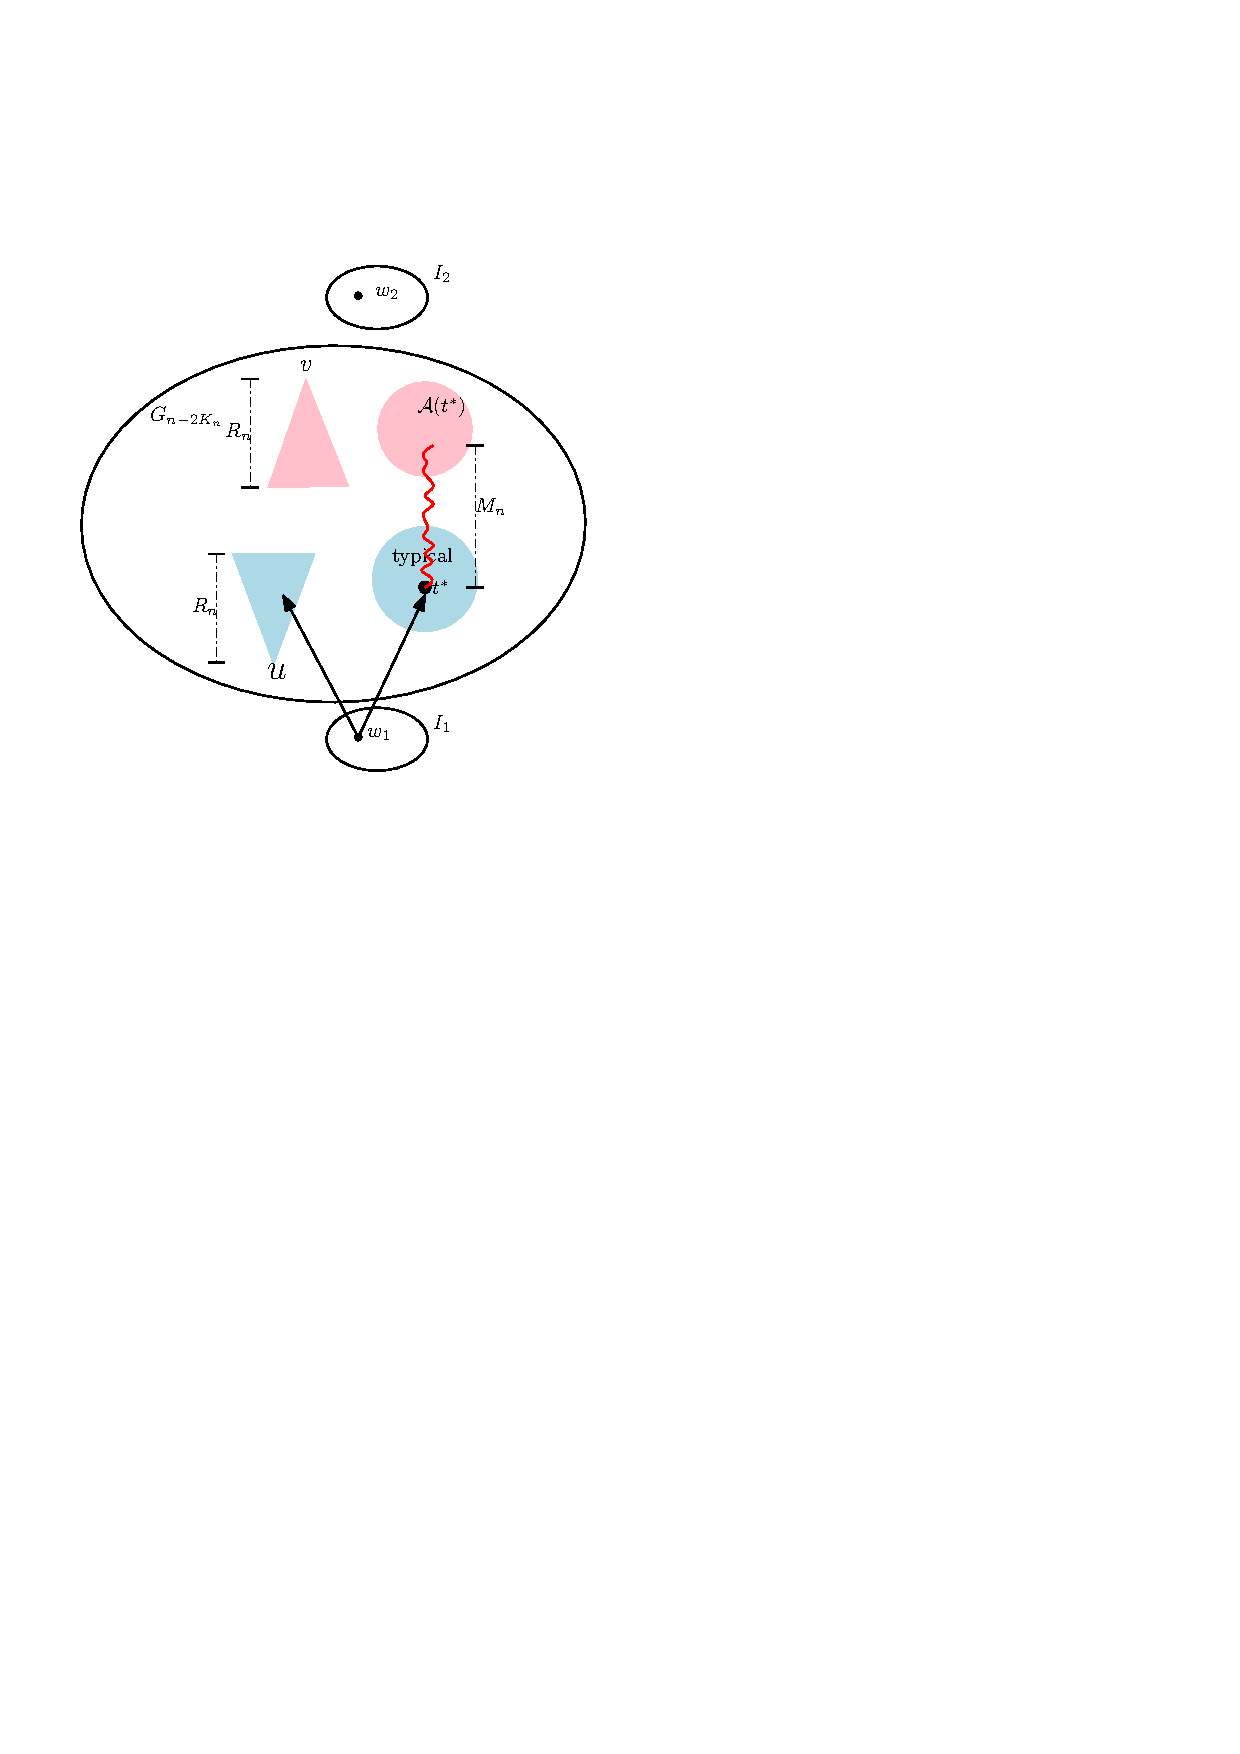
\includegraphics[width=.4\linewidth]{n_minus_2K_5.pdf}}
    
    \only<6>{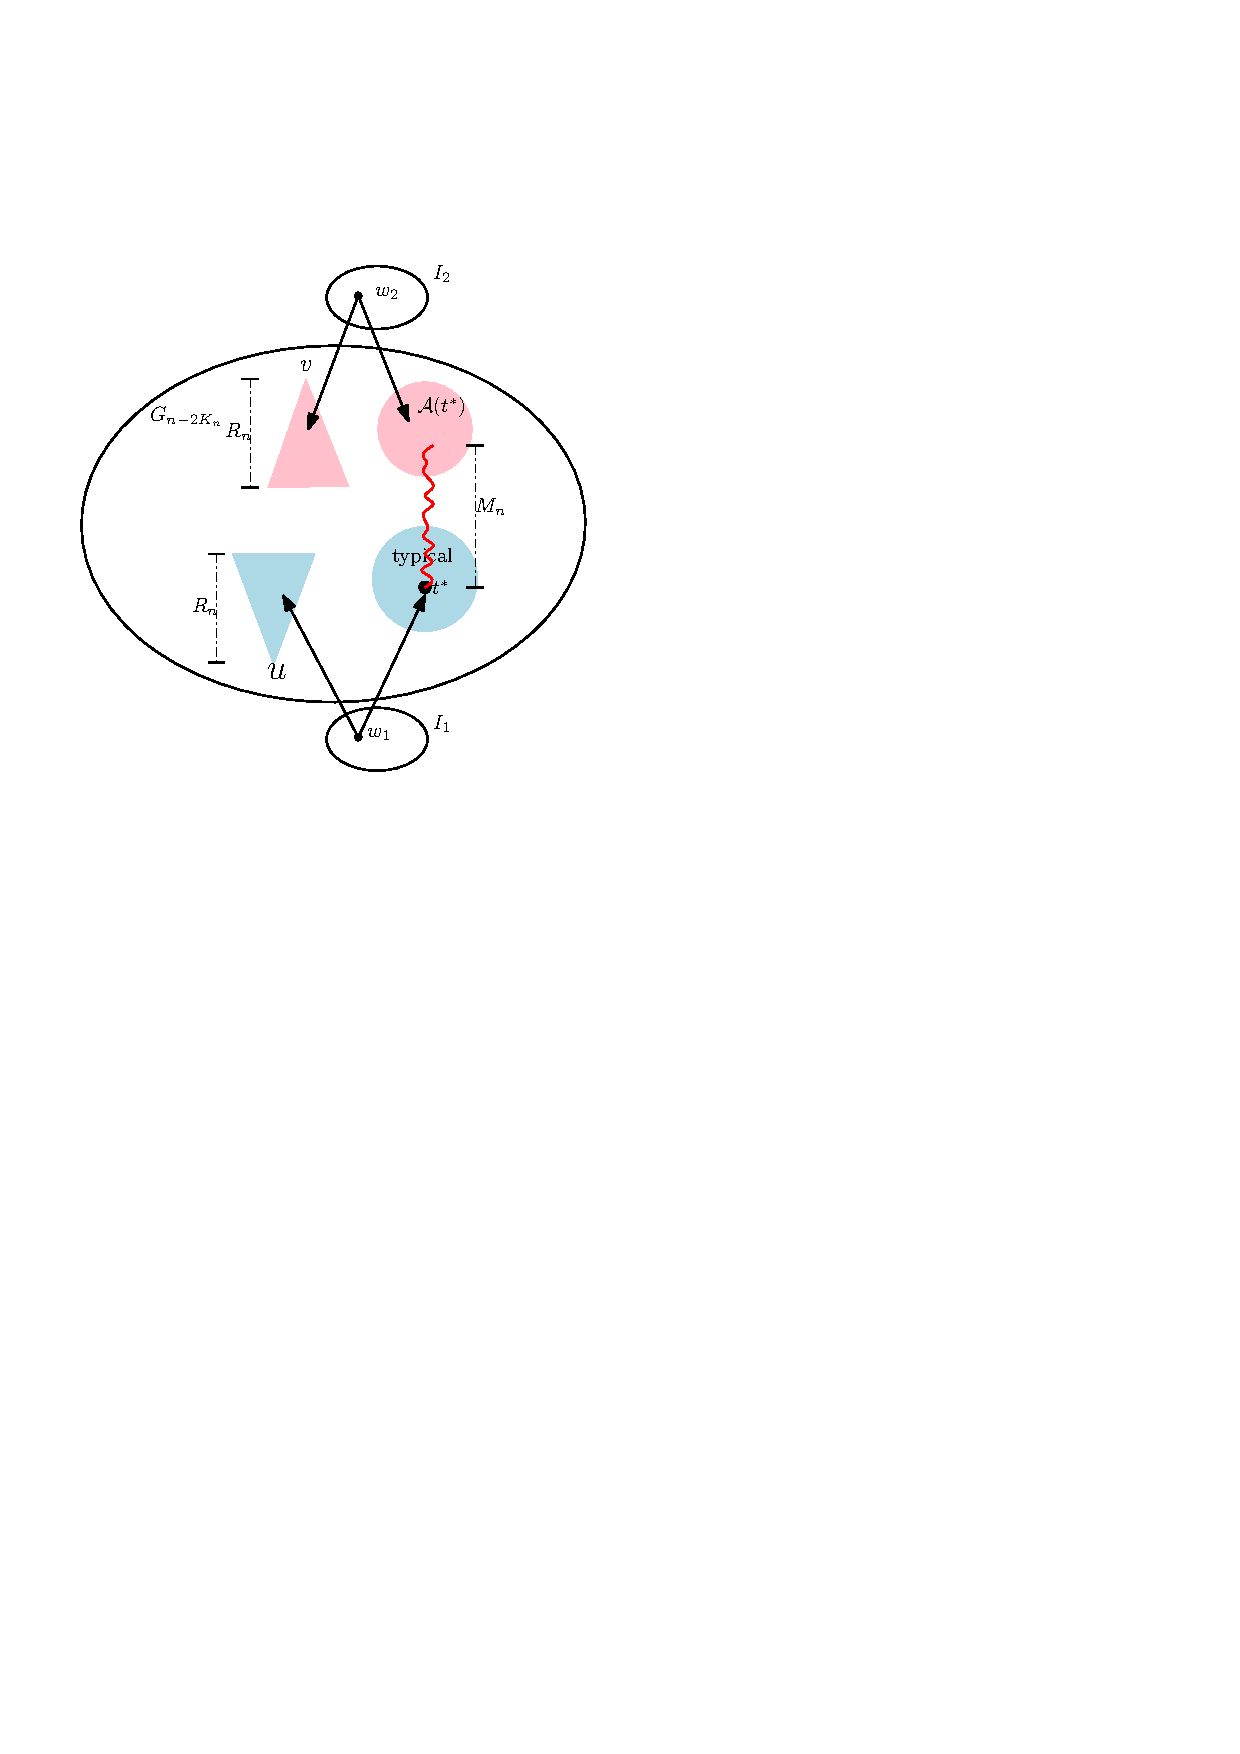
\includegraphics[width=.4\linewidth]{n_minus_2K_6.pdf}}
\end{frame}

\begin{frame}{Tackling the last $2K_n$ vertices}
\footnotesize
	\begin{itemize}
		\item Show for any $u\in [n-2K_n,n]$, $\operatorname{dist}_{G_n}(u,[1,n-2K_n])\leq R_n+2\,.$
		\item \textcolor{blue}{BFS} (breath-first search) in $N_{R_n}(u)$.  $\mathcal F_{k-1}$ as the attachment of $v_1,\dots,v_{k-1}$. 
		\item Applying the conditional attachment lemma, $$\mathbb P\big[ v_k \not\to [1,n-2K_n]\,|\,\mathcal F_{k-1}\big]= O\left(\frac{1}{\log n}\right)\,.$$
		\item  $\mathbb P\Big[ N_{R_n}(u)\cap [1,n-2K_n]=\emptyset \Big]\leq (1/\log n)^{(\log n)^3}=o(1/n^3)$, by \textcolor{blue}{iterative conditioning}.
     	\end{itemize}
        
        \vspace{2mm}
    \centering
    \only<1>{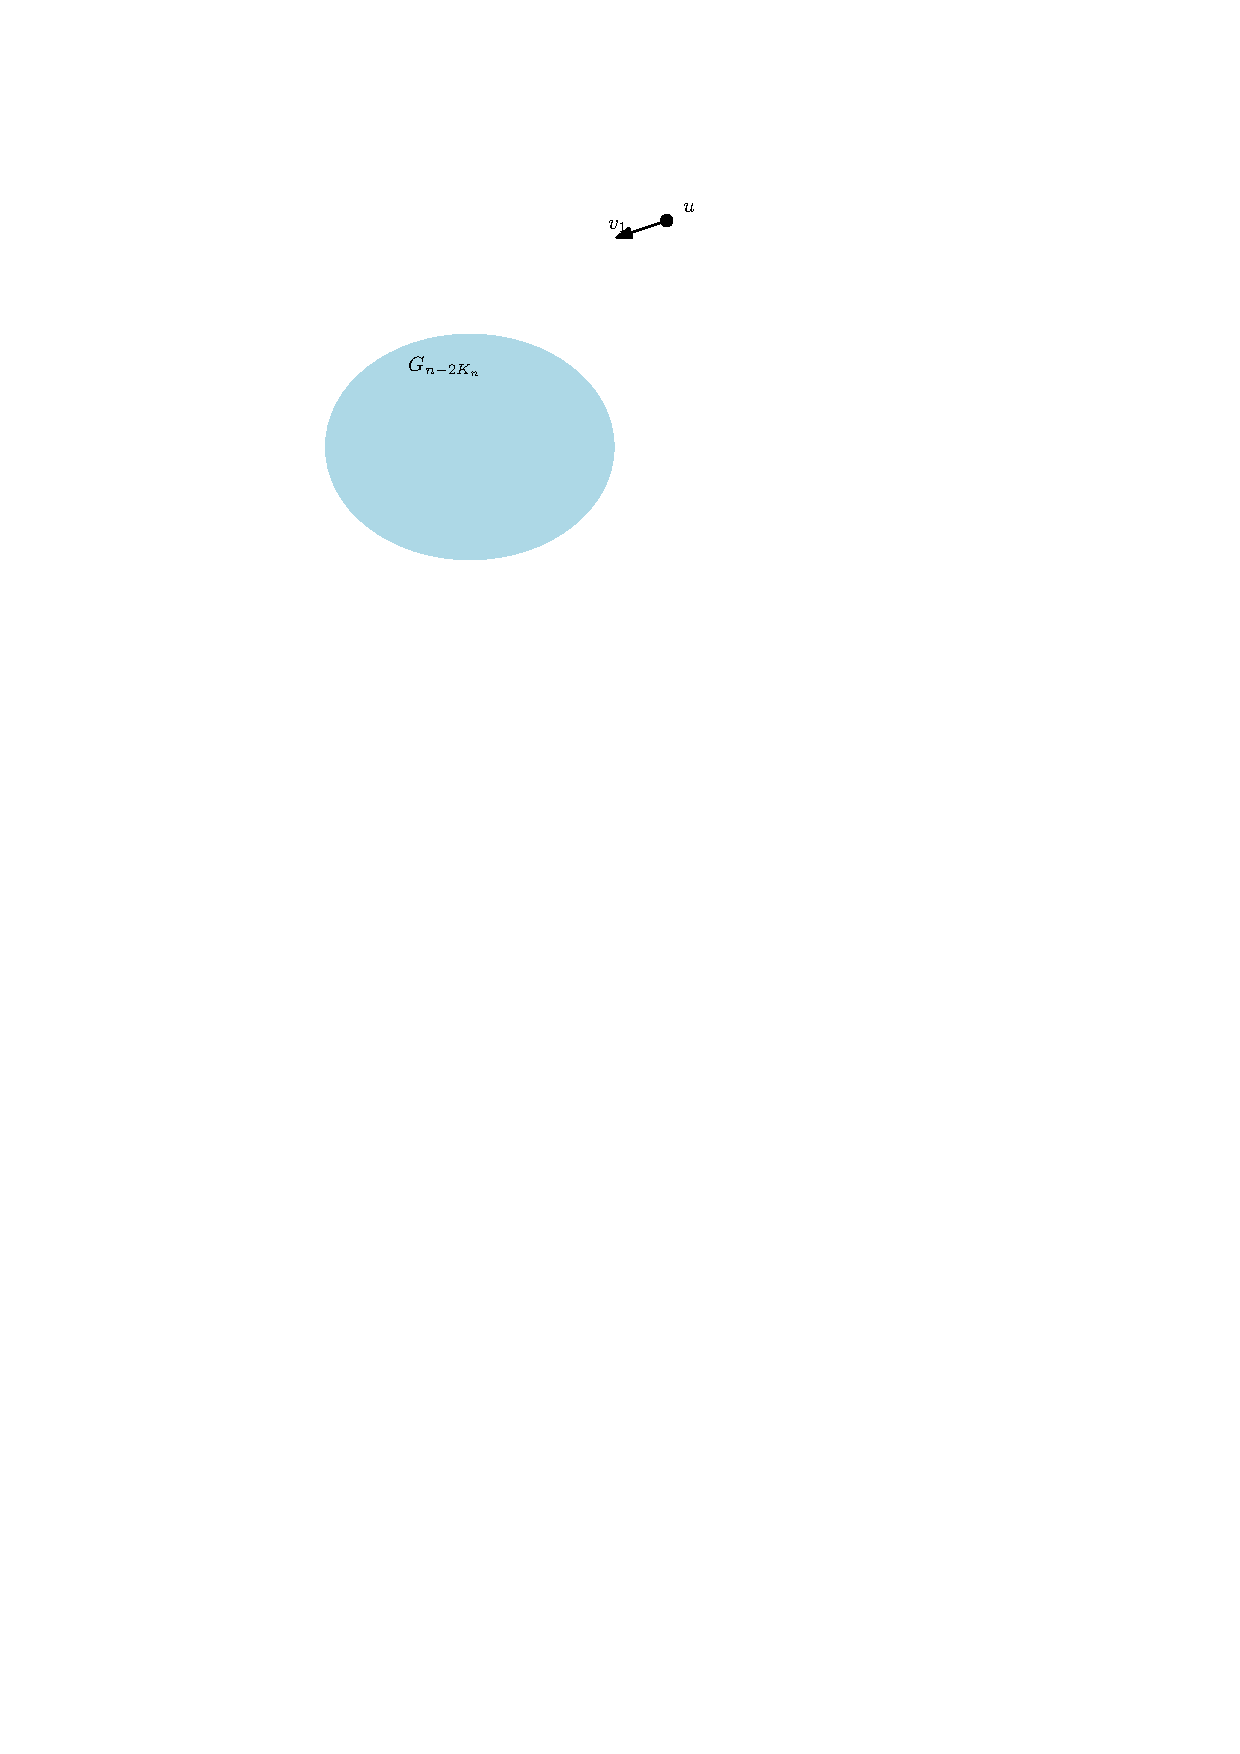
\includegraphics[width=.35\linewidth]{remain_vert_1.pdf}}
    
    \only<2>{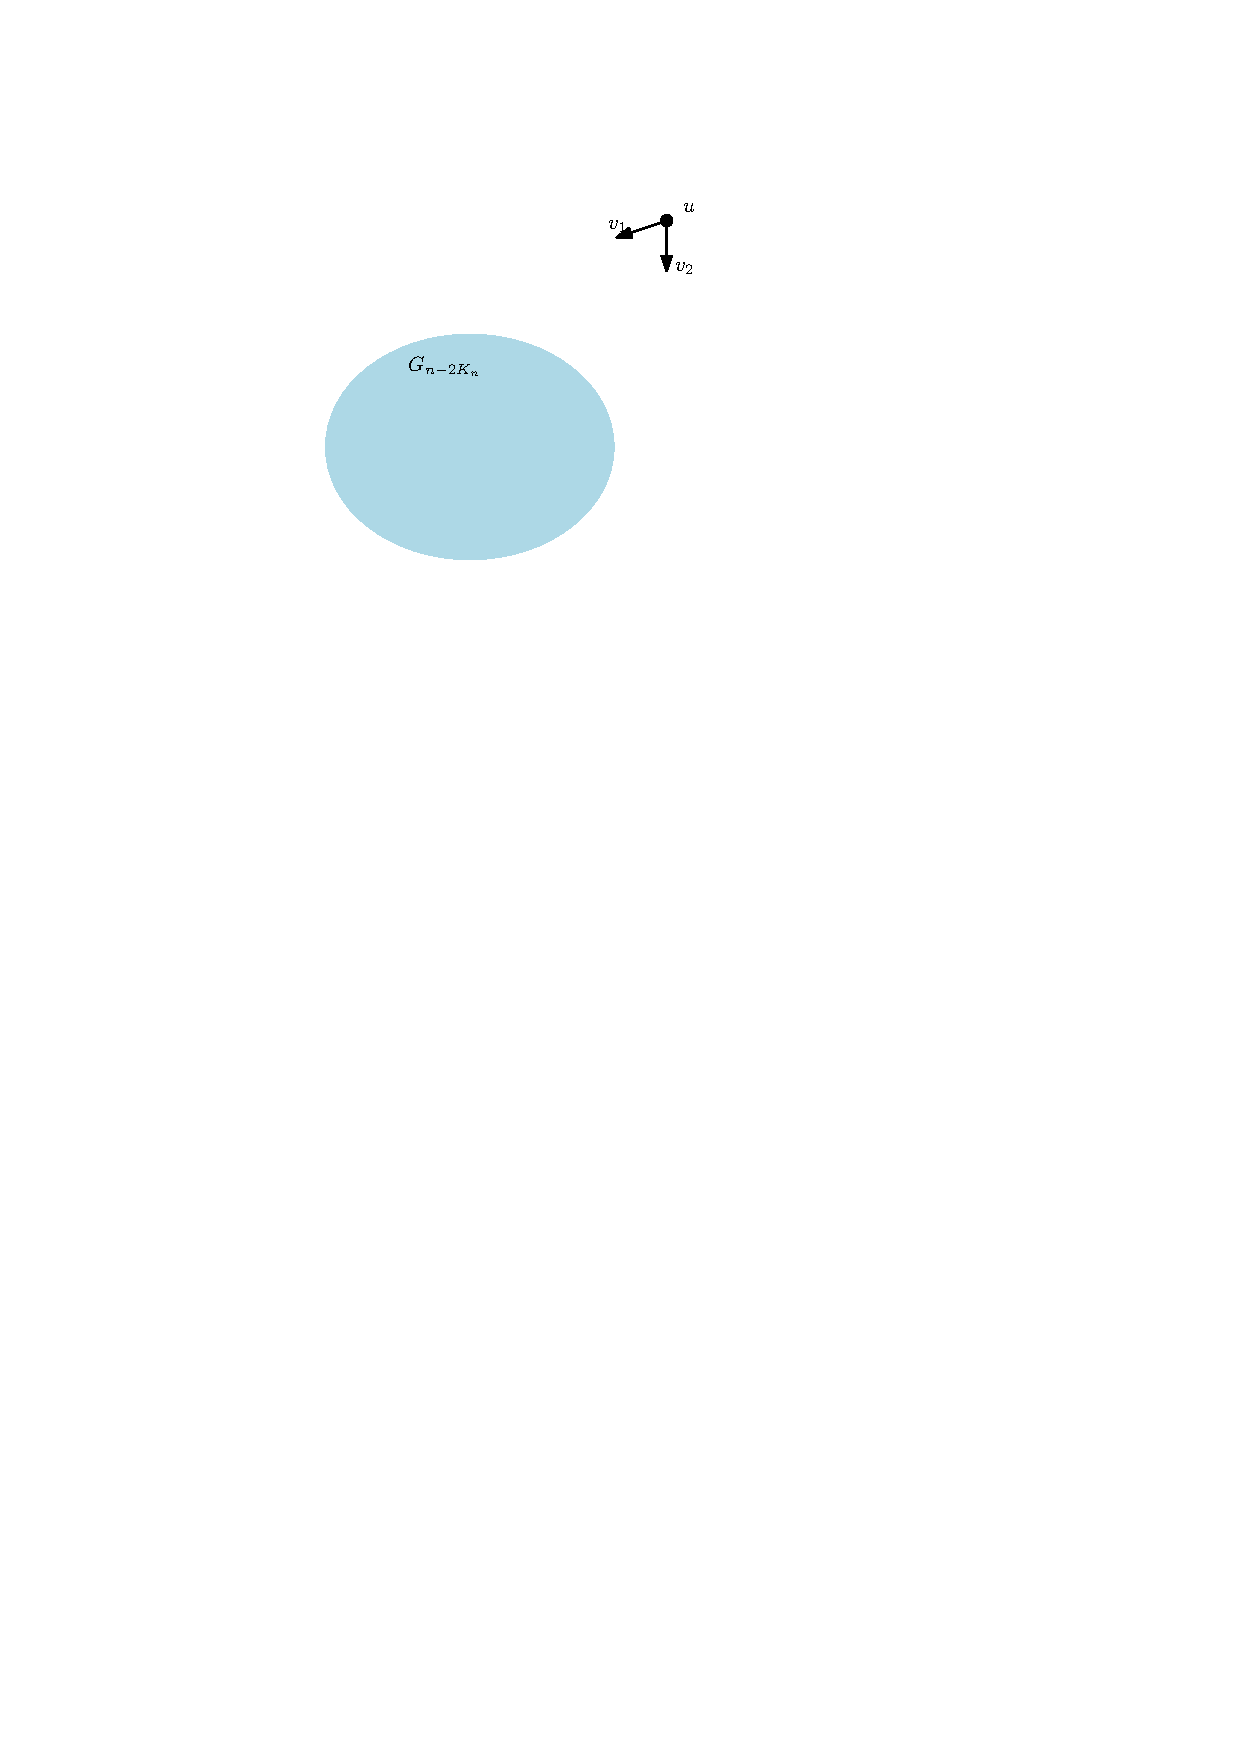
\includegraphics[width=.35\linewidth]{remain_vert_2.pdf}}
    
    \only<3>{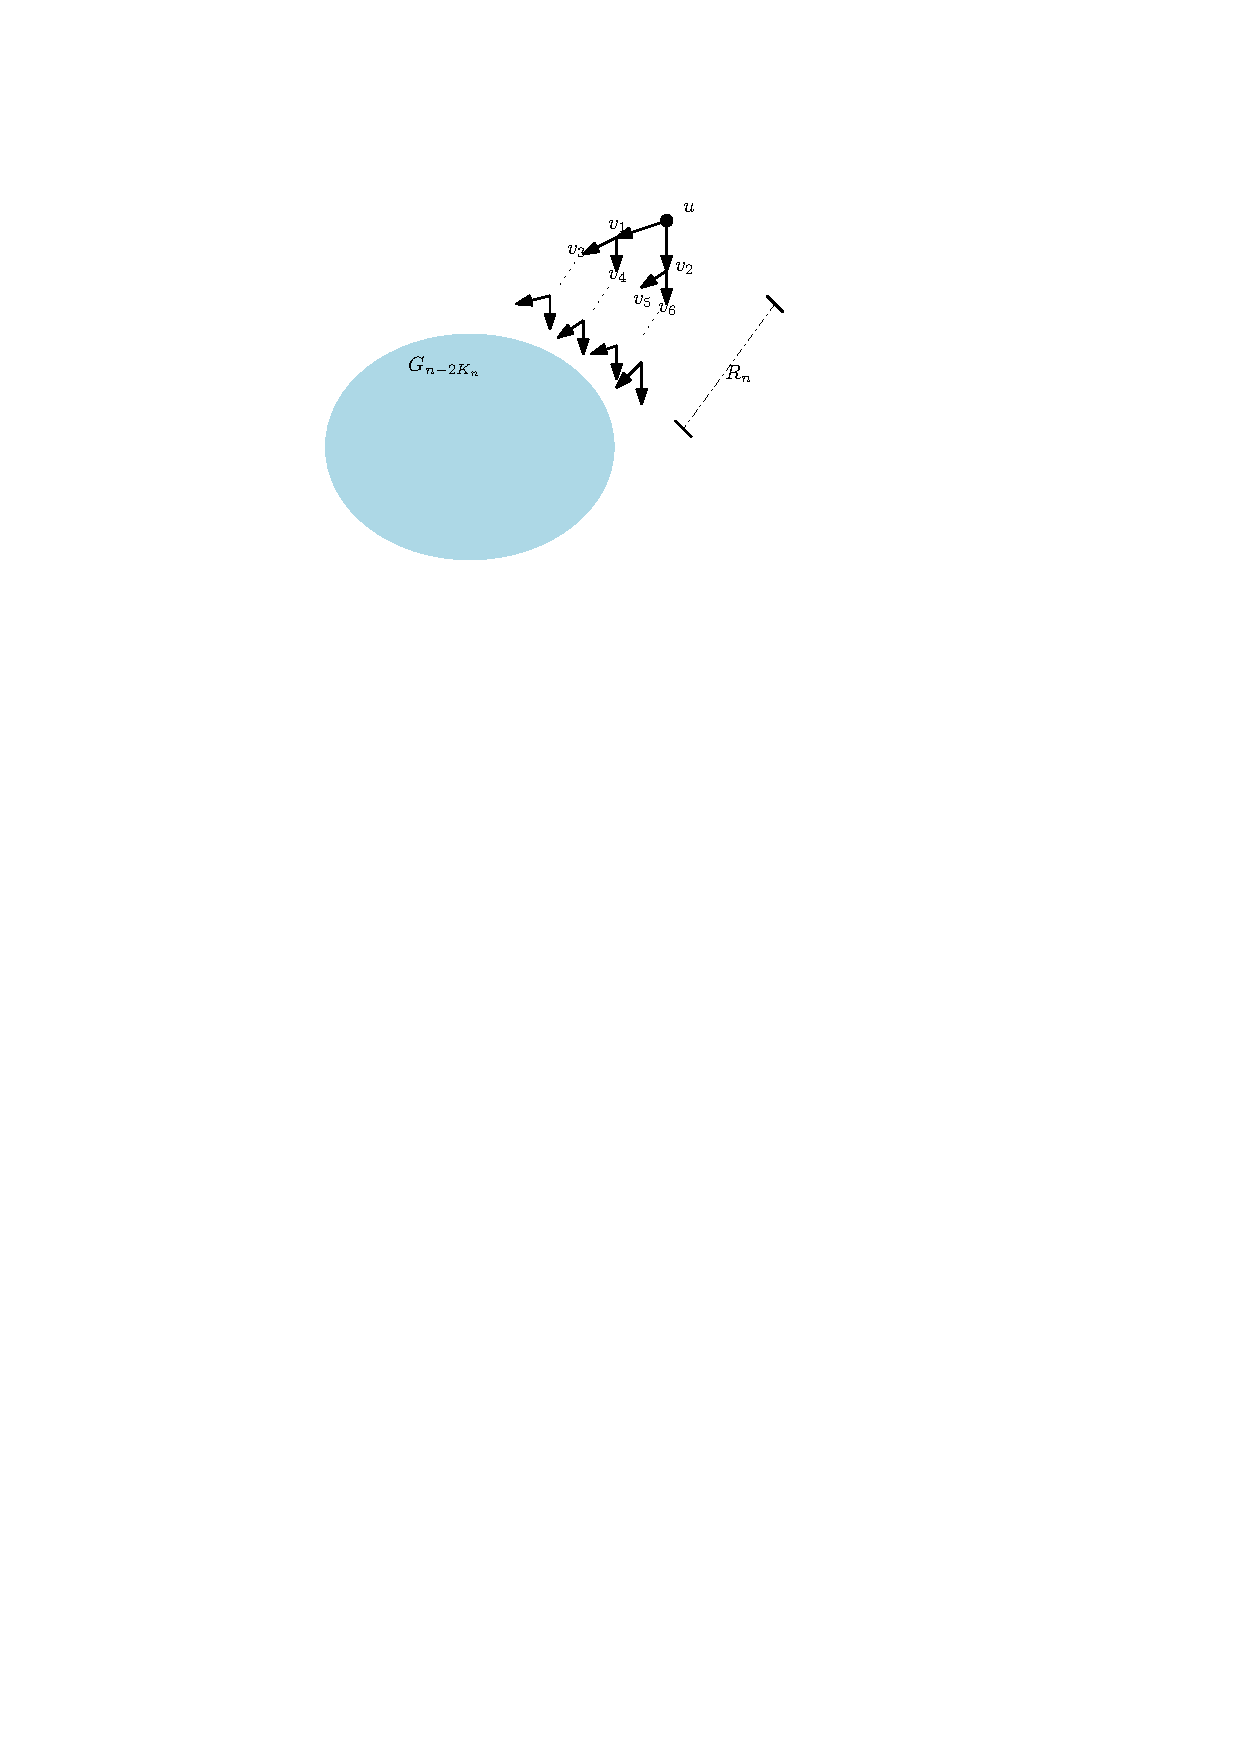
\includegraphics[width=.41\linewidth]{remain_vert_3.pdf}}
    
    \only<4>{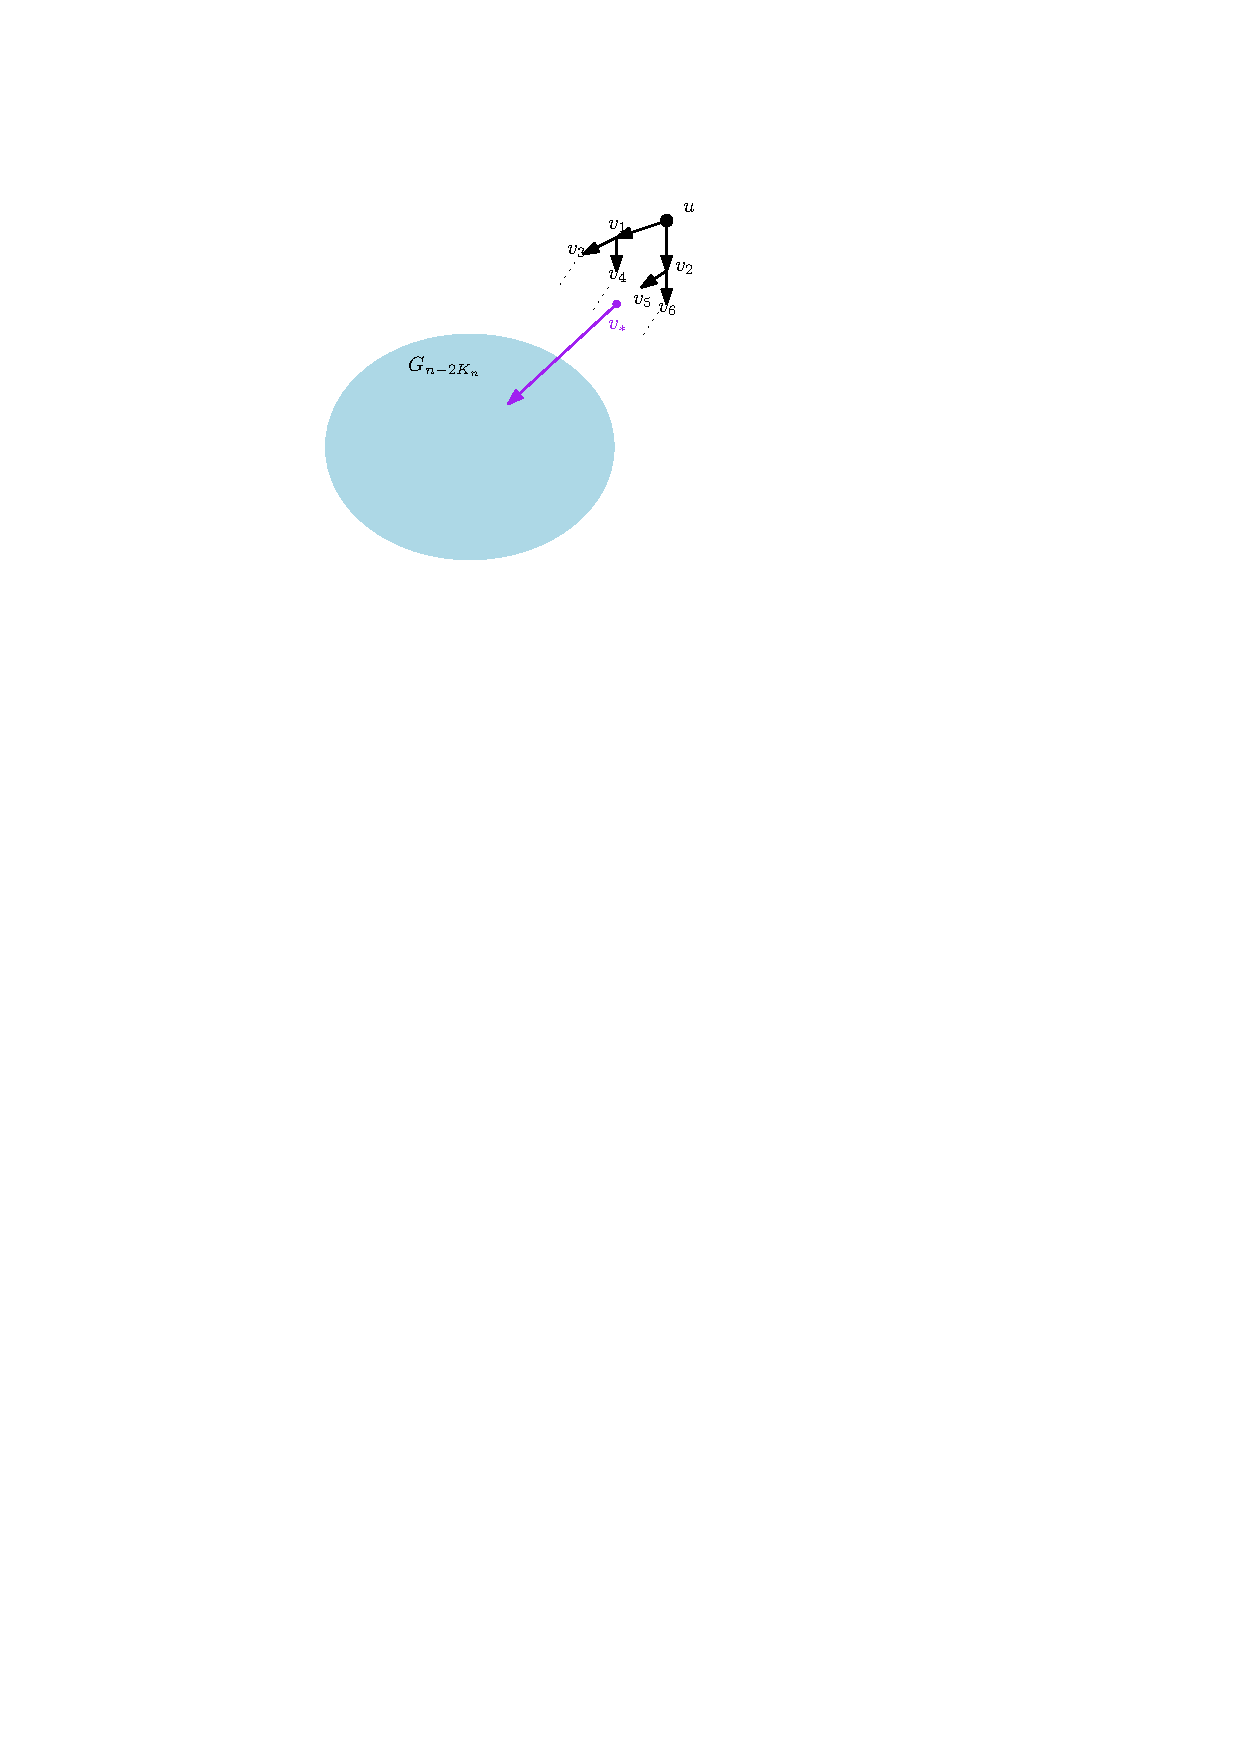
\includegraphics[width=.35\linewidth]{remain_vert_4.pdf}}
\end{frame}

\begin{frame}{Outlook and discussions}
	\begin{itemize}
		\item We prove the asymptotic diameter of the PA model is $\log_\nu n$ when $m\geq 2,\delta>0$.
		\item \textcolor{blue}{End of the story?} We hope the proof technique can be applied to other graph models.
		\item \textcolor{blue}{Open question}: 
        \begin{itemize}
            \item[(1)] Conditional on diameter being $C\log_\nu n$ with $C>1$, what is the graph structure?
            \item[(2)] Pinpointing the second order of the diameter of PA model. \textcolor{blue}{Conjecture}: $\log_\nu n+O(\log\log n)$.
        \end{itemize}
        
	\end{itemize}
	\begin{center}
		\textbf{Thank you!}
	\end{center}
	
\end{frame}



\end{document}